
\section{Modelo de información de In-Help}

\subsection{Descripción general}
 En la figura~\ref{fig:Modelo_Info_In-Help} se muestra la estructura de información que manejará para la implementación del sistema y aplicación In-Help
 
\begin{figure}[htbp!]
	\begin{center}
		\fbox{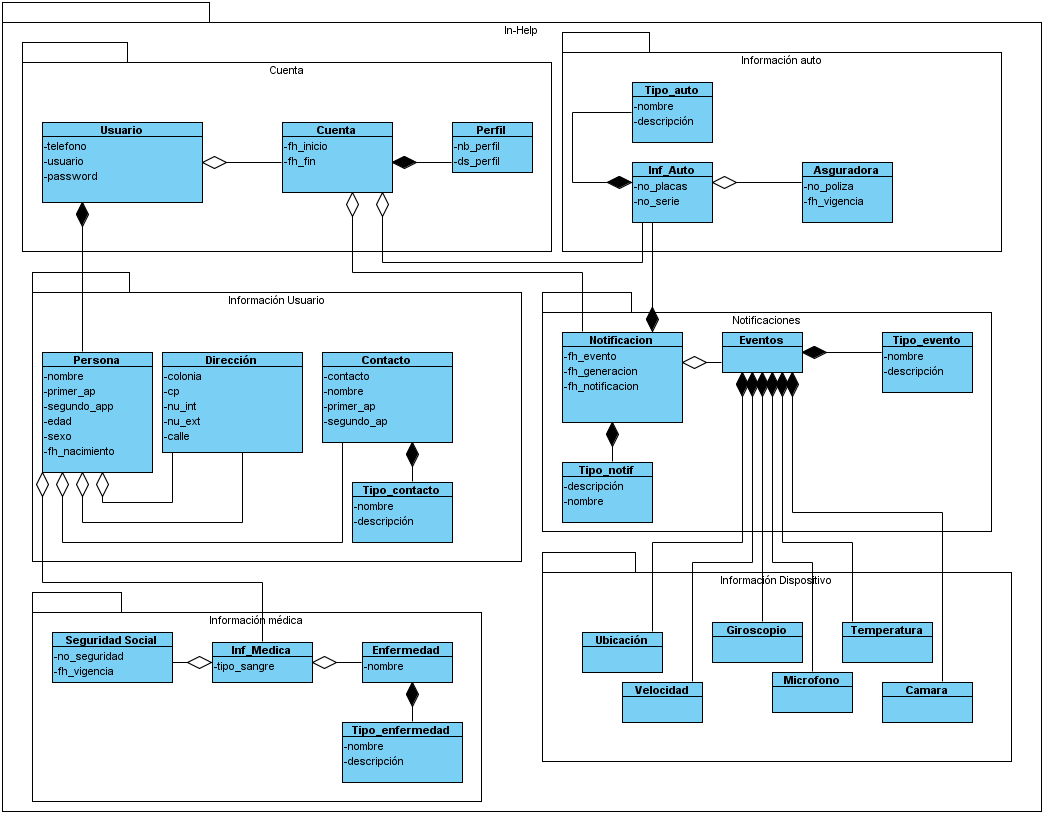
\includegraphics[width=1.1\textwidth]{ModeloNegocios/images/Informacion/DG_Informacion}}
		\caption{Modelo de información In-Help}
		\label{fig:Modelo_Info_In-Help}
	\end{center}
\end{figure}

\begin{BusinessEntity}{Usuario}{Usuario} 
    \Battr{usuario}{Usuario}{\tdCadena}{Es el identificador único para el usuario}{\requerido}{\longitudMinMax{5}{}{30}{}}
    \Battr{password}{Password}{\tdCadena}{Es la clave de acceso del usuario para la aplicación}{\requerido}{\longitudMinMax{8}{}{20}{}}
	\Battr{telefono}{Teléfono}{\tdNumerico}{Es el número de teléfono celular del usuario}{\requerido}{\longitudExacta{10}{}}
\end{BusinessEntity}

\begin{BusinessEntity}{Cuenta}{Cuenta} 
	\Battr{fh_inicio}{Fecha inicio}{\tdFecha}{Es la fecha en la que el usuario creo su cuenta}{\requerido}
	\Battr{fh_fin}{Fecha fin}{\tdFecha}{Es la fecha en la que el usuario elimino su cuenta}{\opcional}
\end{BusinessEntity}

\begin{BusinessEntity}{Perfil}{Perfil} 
	\Battr{nb_perfil}{Nombre de perfil}{\tdPalabra}{Es el nombre que identifica al perfil}{\requerido}{\longitudMinMax{2}{}{30}{}}
	\Battr{ds_perfil}{Es la descripción de perfil}{\tdFrase}{Es la descripción de las actividades del perfil}{\requerido}{\longitudMinMax{10}{}{100}{}}

\end{BusinessEntity}

